\scanpage{20}
% Foliotation archivistique au crayon, en bas à gauche : 19.
\diagram{\begin{tikzcd}[ampersand replacement=\&,column sep=small,row sep=large]
D \arrow[r,phantom,"\subset"] \arrow[d,"\text{fini}"'] \& \mathbb G_m \arrow[dl,no head] \\
\mathbb Q \&
\end{tikzcd}}
\diagram{\begin{tikzcd}[ampersand replacement=\&,row sep=large,column sep=small]
\& \vdots \& \\
\& {}_{\unsure{n}}U \arrow[d,no head] \& \\
\underline{\operatorname{Hom}}(D,\mathbb G_m) \arrow[d,"n"] \arrow[r,phantom,"="] \& U \arrow[d,"n"] \& \xi \\
\underline{\operatorname{Hom}}(D,\mathbb G_m) \arrow[r,phantom,"="] \& U \arrow[d,no head] \& \\
\& \vdots \&
\end{tikzcd}}
\[T(\mathbb Q)\ni\xi\qquad H^1(\mathbb Q,T_\infty(U))\]
\figure{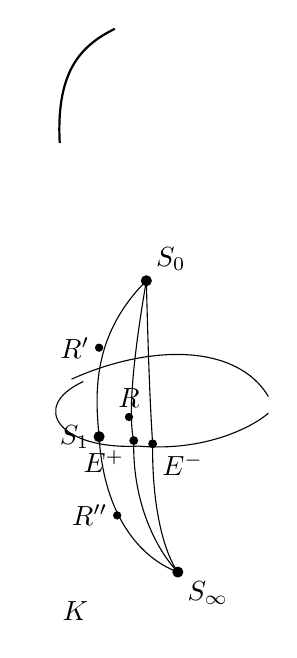
\begin{tikzpicture}[x=1cm,y=1cm]
\draw[line width=.8pt] (-.9,3.25) .. controls (-.95,4.2) and (-.6,4.5) .. (-.2,4.7);
\draw (-.6,.22) .. controls (-1.3,-.1) and (-.9,-.65) .. (.1,-.6)
 .. controls (1.05,-.68) and (1.65,-.28) .. (1.75,-.18);
\draw (-.75,.25) .. controls (.25,.7) and (1.35,.7) .. (1.75,.03);
\draw (.2,1.5) .. controls (-.5,.8) and (-.45,.05) .. (-.4,-.48)
 .. controls (-.34,-1.48) and (.12,-2.02) .. (.6,-2.2);
\draw (.2,1.5) .. controls (.02,.45) and (-.03,-.22) .. (.04,-.53)
 .. controls (.02,-1.35) and (.35,-1.94) .. (.6,-2.2);
\draw (.2,1.5) .. controls (.22,.72) and (.24,.04) .. (.28,-.57)
 .. controls (.27,-1.45) and (.45,-1.99) .. (.6,-2.2);
\fill (.2,1.5) circle (2pt) node[above right] {$S_0$};
\fill (-.4,-.48) circle (2pt) node[left] {$S_1$};
\fill (.6,-2.2) circle (2pt) node[below right] {$S_\infty$};
\fill (-.4,.65) circle (1.5pt) node[left] {$R'$};
\fill (-.17,-1.48) circle (1.5pt) node[left] {$R''$};
\fill (.04,-.53) circle (1.6pt) node[below left] {$E^+$};
\fill (.28,-.57) circle (1.6pt) node[below right] {$E^-$};
\fill (-.02,-.23) circle (1.5pt) node[above] {$R$};
\node at (-.7,-2.7) {$K$};
\end{tikzpicture}}
\diagram{\begin{tikzcd}[ampersand replacement=\&,column sep=huge,row sep=large]
\Gamma \arrow[r] \arrow[dr,"{\text{image de dim }\unsure{n+1|11+1}\ ?}"'] \& \operatorname{Aff}(T_\infty(U)) \arrow[d] \\
\& \operatorname{Aut}(T_\infty(U))
\end{tikzcd}}
Ss-grpe d'indice fini : opère par homothéties

$\unsure{\xi_i|\zeta_i}$ --- $\unsure{\mathbb Z}$-indép. mod racines de $1$
\diagram{\begin{tikzcd}[ampersand replacement=\&,column sep=large,row sep=large]
\Gamma \arrow[r] \arrow[dr] \& \operatorname{Aff}(n,\widehat{\mathbb Z}) \arrow[d] \\
\& \widehat{\mathbb Z}^{*}\cdot\widehat{\mathbb Z}^{n}
\end{tikzcd}}
\deleted{image de}
\margin{image d'indice fini ???}
